\specialsection{Community}{}{black}{white}
\subsection{A distributed community}

% \subsection{Recommendations for Future Research}
% \subsection{Recommendations for Future Research}
% \subsection{Recommendations for Future Research}
Ben Fry is the most active forum contributor, but the activity distribution is more balanced than in Git commits, possibly due to the diverse topics covered, including technical queries and bugs. A total of 1,039 individuals contributed to the forum discussions as shown in Figure~\ref{fig:processing-alpha-dot}.

Casey Reas suggests that from 2002 to 2006, the forum cultivated a "unified international community" \parencite[331]{conradGraphicDesignPostdigital2021}. 


% todo create a whole new document that is jsut this size
% Start a new page with a new size
\clearpage
% \pdfpagewidth=\diagramPaperWidth % New width for the following pages
% \pdfpageheight=\paperHeight % New height for the following pages

\begin{figure}[h!]
  \centering
  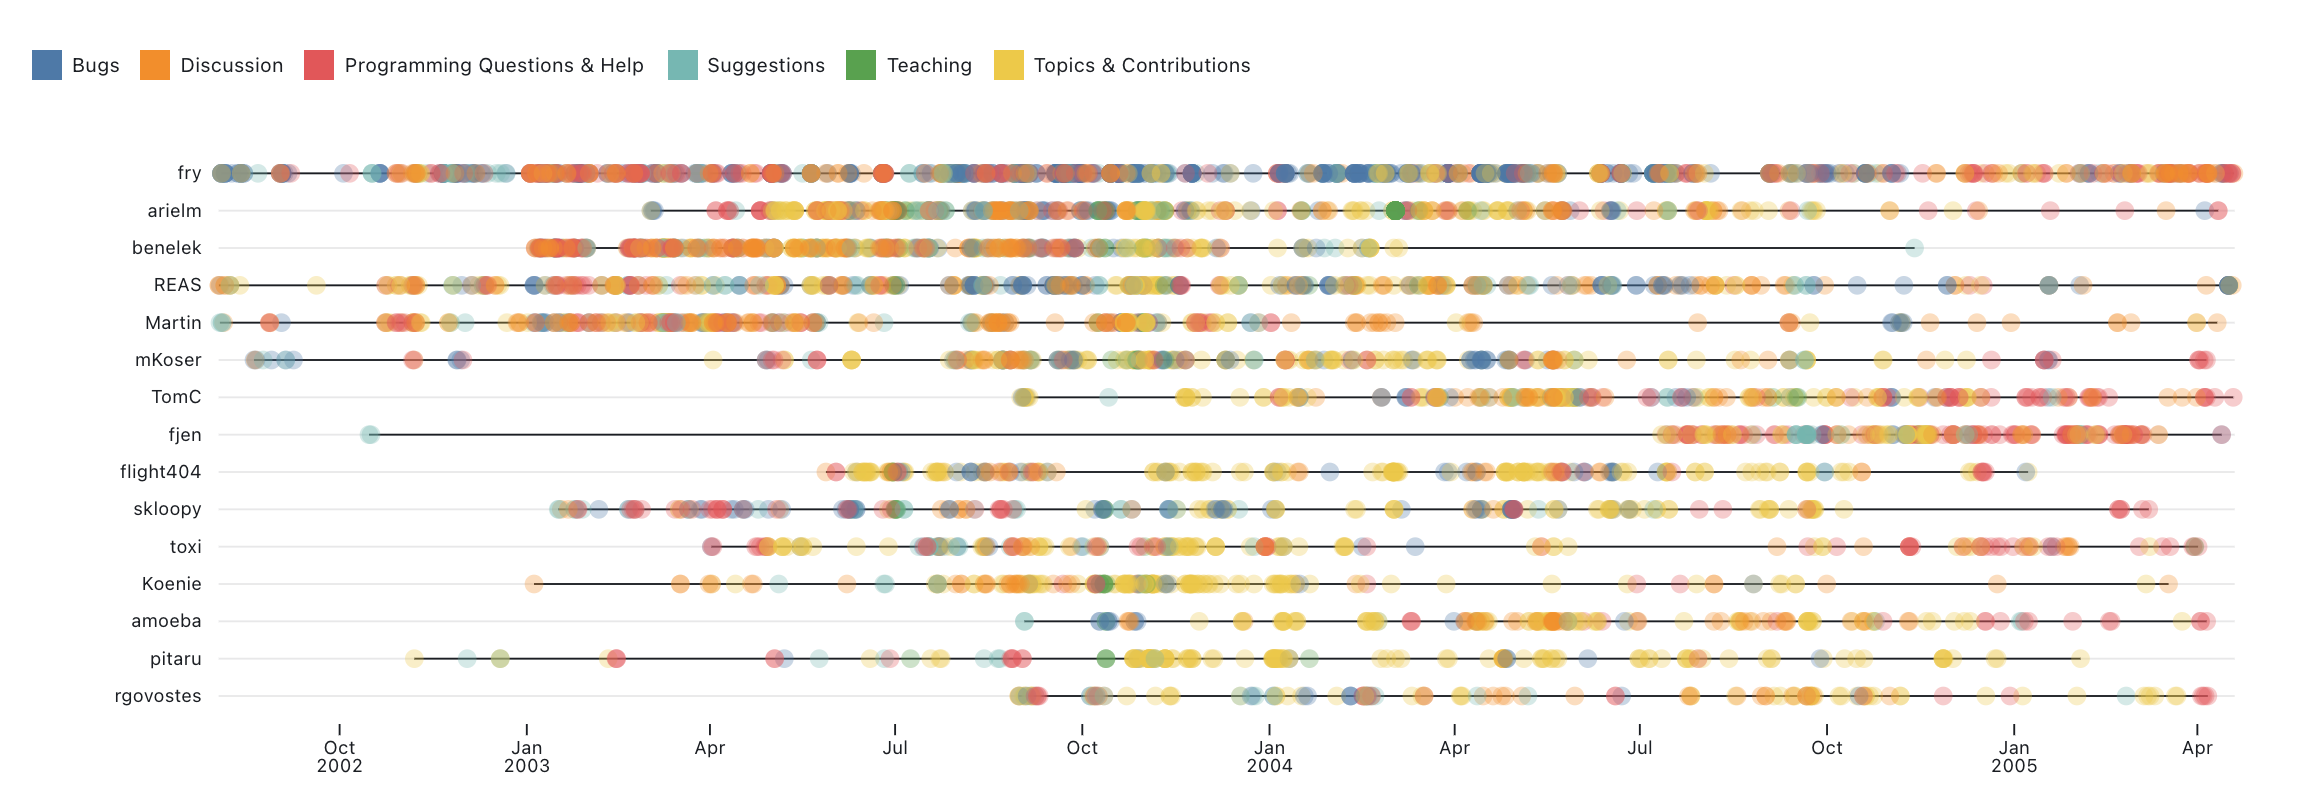
\includegraphics[width=1.0\textwidth]{images/alpha-forum-top15.png}
  \caption{Posting activity of the 15 most active contributors on the alpha forum.}
  \label{fig:processing-alpha-dot}
\end{figure}

% Revert to the original size
\clearpage

% \pdfpagewidth=\paperWidth % Width of A4 paper
% \pdfpageheight=\paperHeight % New height for the following pages
% \clearpage
% \restoregeometry


Linus's Law—"Given enough eyeballs, all bugs are shallow" \parencite[29]{raymondCathedralBazaar1999}—is somewhat evidenced by increased forum activity during release periods, suggesting community involvement in bug identification, as demonstrated in Figure~\ref{figure:forum-git-activity}.

\begin{figure}[!htbp] 
    \centering 
    %\includesvg[pretex=\sffamily\fontsize{5.58pt}{8pt}\selectfont, width=1\textwidth, keepaspectratio]{images/figure-forum-git-activity.png}
    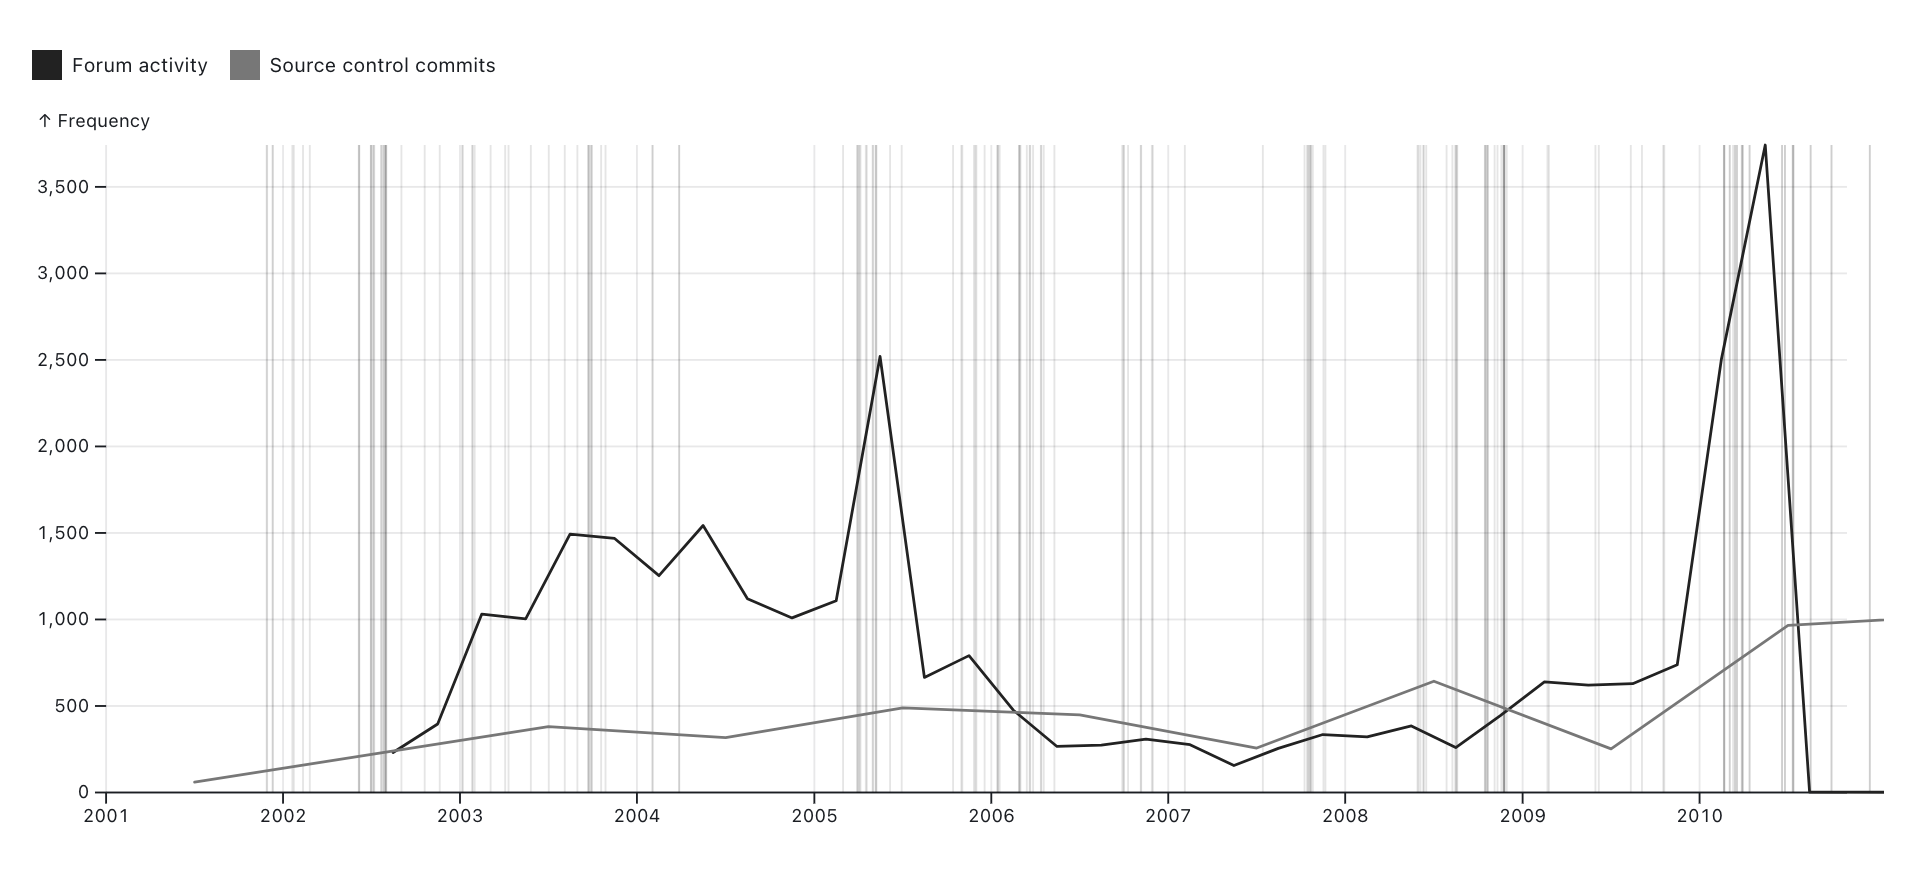
\includegraphics[width=1\textwidth]{images/figure-forum-git-activity.png} 

    \caption{Forum vs git activity vs releases (vertical lines)}
    \label{figure:forum-git-activity}  
  \end{figure}

Contrary to the initial assumption that primary contributors would predominantly be from the MIT ACG group, given the project's origins, a preliminary analysis suggests otherwise.

\begin{figure}[htbp]
  \centering
  
  % Row 1
  \begin{subfigure}[b]{0.24\textwidth}
      \includesvg[pretex=\sffamily\fontsize{5.58pt}{8pt}\selectfont, width=1\textwidth, keepaspectratio]{images/month1.svg}
      \caption{Month 1}
      \label{fig:month1}
  \end{subfigure}
  \hfill
  \begin{subfigure}[b]{0.24\textwidth}
    \includesvg[pretex=\sffamily\fontsize{5.58pt}{8pt}\selectfont, width=1\textwidth, keepaspectratio]{images/month2.svg}
      \caption{Month 2}
      \label{fig:month2}
  \end{subfigure}
  \hfill
  \begin{subfigure}[b]{0.24\textwidth}
    \includesvg[pretex=\sffamily\fontsize{5.58pt}{8pt}\selectfont, width=1\textwidth, keepaspectratio]{images/month3.svg}
      \caption{Month 3}
      \label{fig:month3}
  \end{subfigure}
  \hfill
  \begin{subfigure}[b]{0.24\textwidth}
    \includesvg[pretex=\sffamily\fontsize{5.58pt}{8pt}\selectfont, width=1\textwidth, keepaspectratio]{images/month4.svg}
      \caption{Month 4}
      \label{fig:month4}
  \end{subfigure}
  
  % Add space between rows
  \vspace{0.25cm}

  % Row 2
  \begin{subfigure}[b]{0.24\textwidth}
    \includesvg[pretex=\sffamily\fontsize{5.58pt}{8pt}\selectfont, width=1\textwidth, keepaspectratio]{images/month5.svg}
      \caption{Month 5}
      \label{fig:month5}
  \end{subfigure}
  \hfill
  \begin{subfigure}[b]{0.24\textwidth}
    \includesvg[pretex=\sffamily\fontsize{5.58pt}{8pt}\selectfont, width=1\textwidth, keepaspectratio]{images/month6.svg}
      \caption{Month 6}
      \label{fig:month6}
  \end{subfigure}
  \hfill
  \begin{subfigure}[b]{0.24\textwidth}
    \includesvg[pretex=\sffamily\fontsize{5.58pt}{8pt}\selectfont, width=1\textwidth, keepaspectratio]{images/month7.svg}
      \caption{Month 7}
      \label{fig:month 7}
  \end{subfigure}
  \hfill
  \begin{subfigure}[b]{0.24\textwidth}
    \includesvg[pretex=\sffamily\fontsize{5.58pt}{8pt}\selectfont, width=1\textwidth, keepaspectratio]{images/month8.svg}
      \caption{Month 8}
      \label{fig:month 8}
  \end{subfigure}

  % Add space between rows
  \vspace{0.25cm}

  % Row 3
  \begin{subfigure}[b]{0.24\textwidth}
    \includesvg[pretex=\sffamily\fontsize{5.58pt}{8pt}\selectfont, width=1\textwidth, keepaspectratio]{images/month9.svg}
      \caption{Month 9}
      \label{fig:month9}
  \end{subfigure}
  \hfill
  \begin{subfigure}[b]{0.24\textwidth}
    \includesvg[pretex=\sffamily\fontsize{5.58pt}{8pt}\selectfont, width=1\textwidth, keepaspectratio]{images/month10.svg}
      \caption{Month 10}
      \label{fig:month10}
  \end{subfigure}
  \hfill
  \begin{subfigure}[b]{0.24\textwidth}
    \includesvg[pretex=\sffamily\fontsize{5.58pt}{8pt}\selectfont, width=1\textwidth, keepaspectratio]{images/month11.svg}
      \caption{Month 11}
      \label{fig:month11}
  \end{subfigure}
  \hfill
  \begin{subfigure}[b]{0.24\textwidth}
    \includesvg[pretex=\sffamily\fontsize{5.58pt}{8pt}\selectfont, width=1\textwidth, keepaspectratio]{images/month12.svg}
      \caption{Month 12}
      \label{fig:month12}
  \end{subfigure}
  
  \caption{Monthly graphs}
  \label{fig:monthlyGraphs}
\end{figure}


\begin{figure}[h!] 
  \centering 
  \includesvg[pretex=\sffamily\fontsize{5.58pt}{8pt}\selectfont, width=1\textwidth, keepaspectratio]{images/year.svg}
  \caption{Year}
  \label{figure:year}  
\end{figure}


%\begin{figure}[h!] 
    \centering 
    \includesvg[pretex=\sffamily\fontsize{5.58pt}{8pt}\selectfont, width=1\textwidth, keepaspectratio]{images/figure-forum-posts.svg}
    \caption{Top 12 authors by number of posts (Aggregated alpha and beta forum)}
    \label{fig:forum-posts}  
  \end{figure}

%\begin{figure}[htbp] 
    \centering
    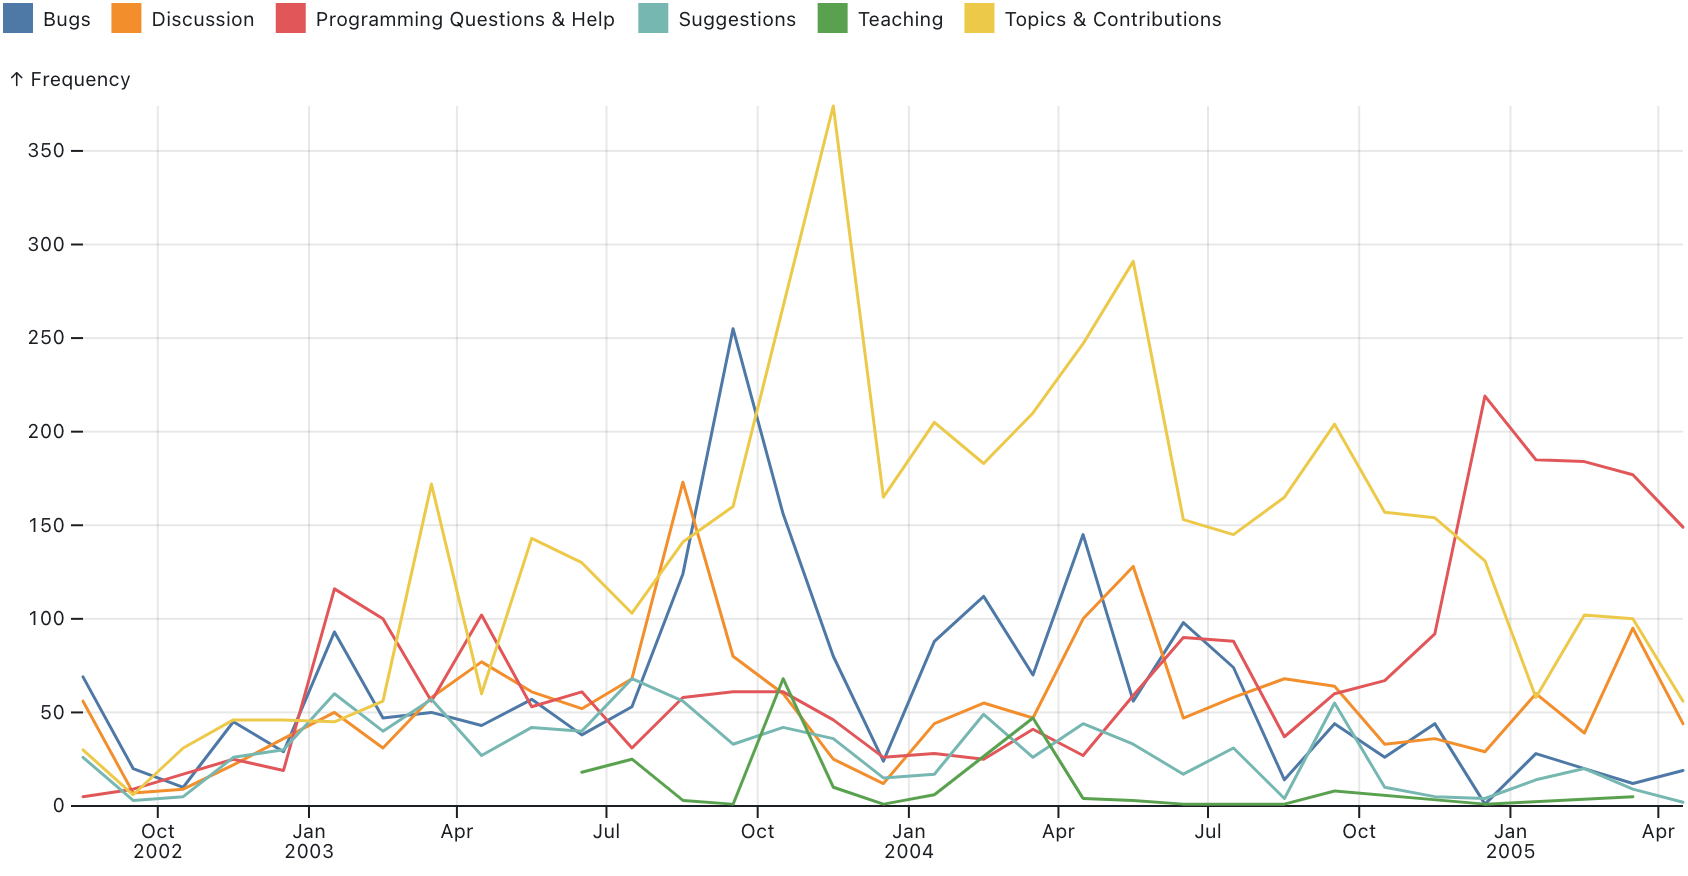
\includegraphics[width=1\textwidth]{alpha-forums-activity.png} 
    % \includesvg[pretex=\sffamily\fontsize{5.58pt}{8pt}\selectfont, width=0.6\textwidth]{images/alpha-forums-activity.svg}
    \caption{Forums activity}
    \label{fig:forum-activity}  
  \end{figure}

%\begin{figure}[h!] 
    \centering 
    \includesvg[pretex=\sffamily\fontsize{5.58pt}{8pt}\selectfont, width=1\textwidth, keepaspectratio]{images/figure-alltime-sourcecode-commits.svg}
    \caption{Top 25 source code contributors by number of commits}
    \label{fig:alltime-sourcecode-commits}  
  \end{figure}

%\begin{figure}[htbp] 
    \centering
    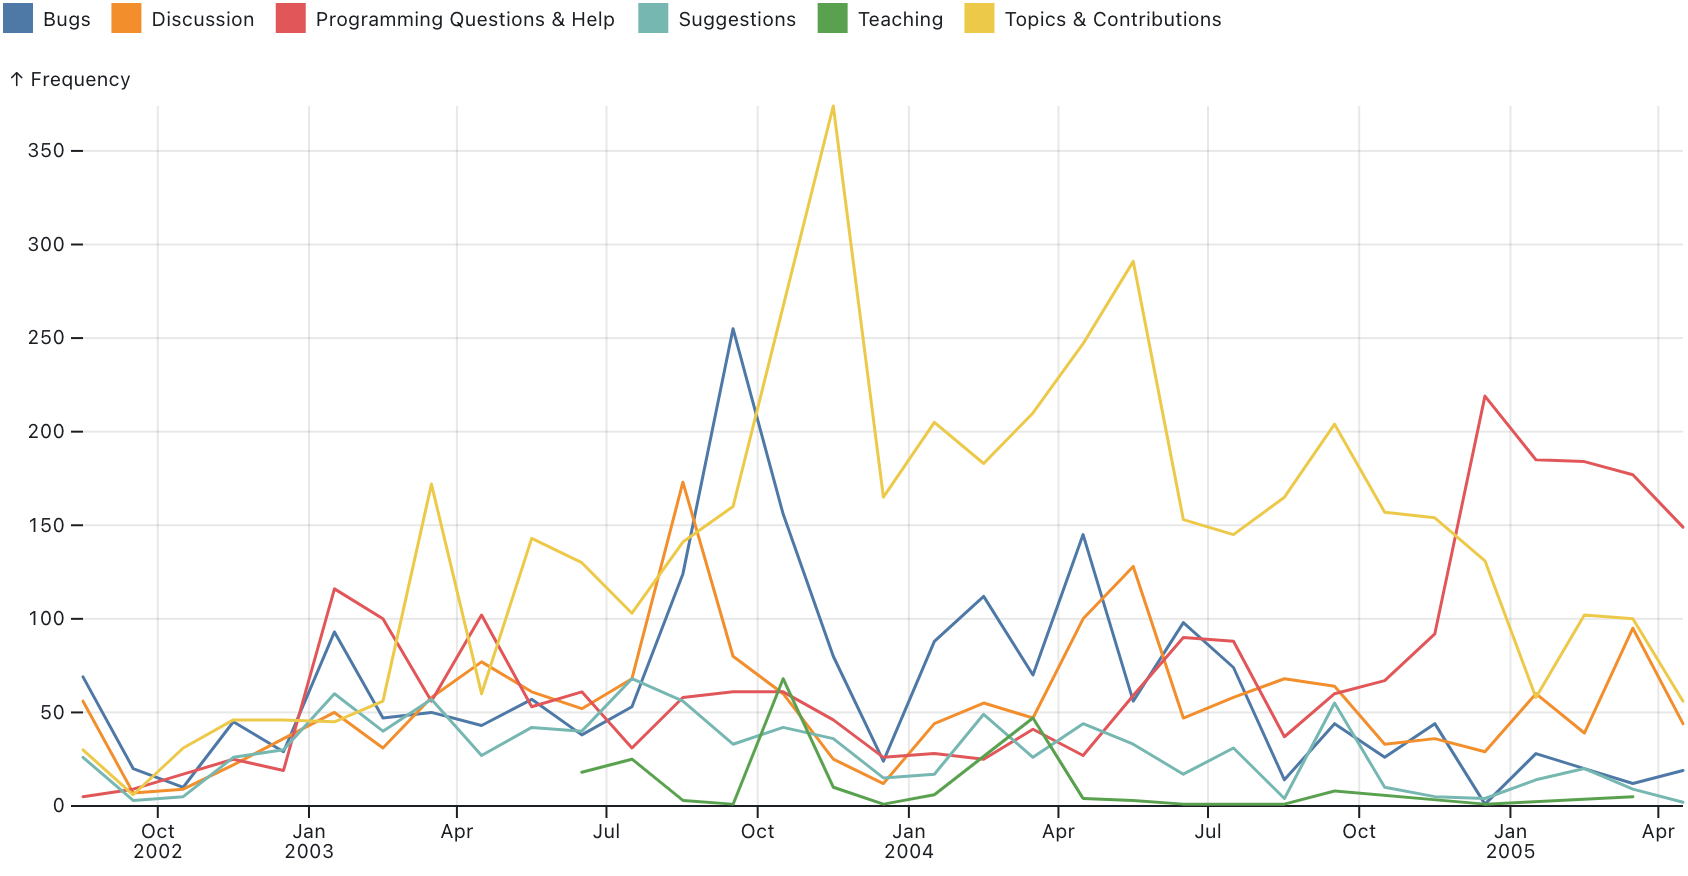
\includegraphics[width=1\textwidth]{alpha-forums-activity.png} 
    % \includesvg[pretex=\sffamily\fontsize{5.58pt}{8pt}\selectfont, width=0.6\textwidth]{images/alpha-forums-activity.svg}
    \caption{Forums activity}
    \label{fig:forum-activity}  
  \end{figure}

% \subsubsection{Synthesized Data Analysis: Git Commits, Releases, and Forum Activity}

% \newpage
% \subsubsection{Alpha Forum Patterns in Forum Contributions (to remove)}
There were 11,926 posts across 2,626 topics from 02/08/2002, 15:29 to the 19/04/2005, 09:55 across 1039 authors in the forum.

The alpha forum was a YaBB (Yet another Bulletin Board), it was seperated into forums which conained boards which contained topics which contained posts.

\begin{figure}
    \centering 
    \includesvg[pretex=\sffamily\fontsize{5.58pt}{8pt}\selectfont, width=1\textwidth, keepaspectratio]{images/alpha-forums-by-posts.svg}
    \caption{Topics by post number}
    \label{fig:forums}  
  \end{figure}

% todo add
% \subsection{Qualitative Insights}
% \subsubsection{Themes from the Forum}
% \subsubsection{Interview Highlights and Key Takeaways}

% \section{Discussion}

% \subsection{Integrating Quantitative and Qualitative Findings}
% \subsection{Implications for the Open Source Community}
% \subsection{The Unique Case of Processing and Creative Coding}
% \subsection{Limitations of the Study}

% \section{Conclusion and Recommendations}

% \subsection{Recap of Key Findings}
% \subsection{Practical Implications for Open Source Projects}
% \subsection{Recommendations for Future Research}



\subsubsection*{Evolution of Community Discussion Platforms}
In the early days of the Processing project, community interactions predominantly took place on forums. These forums served as a primary channel for users to share experiences, discuss problems, and seek help. Notably, the forum discussions underwent significant transformations in terms of platforms over the years, as can be observed in Table \ref{table:forums}. \parencite{ProcessingForum}

\begin{table}[h]
    \raggedright
    \caption{Archival forums composition}
    \label{table:forums}
    \begin{tabular}{l l l c}
        \toprule
        Forum name & Years & URL \\
        \midrule
        Processing alpha forum & 2002-2005 & \href{https://forum.processing.org/alpha/}{forum.processing.org/alpha} \\
        Processing beta forum & 2005-2010 & \href{https://forum.processing.org/beta/}{forum.processing.org/beta}  \\
        Processing 1.0 forum & 2010-2013 & \href{https://forum.processing.org/one/}{forum.processing.org/one} \\
        Processing 2.0 and 3.0 forum & 2013-2018 & \href{https://forum.processing.org/two/}{forum.processing.org/two} \\
        Current processing forum & 2018 - now & \href{https://discourse.processing.org/}{discourse.processing.org} \\
        \bottomrule
    \end{tabular}
  \end{table}

This dynamic shift from one platform to another indicates an evolving user-base and a growing set of needs and tools that community members require for effective collaboration.

% \begin{figure}
%     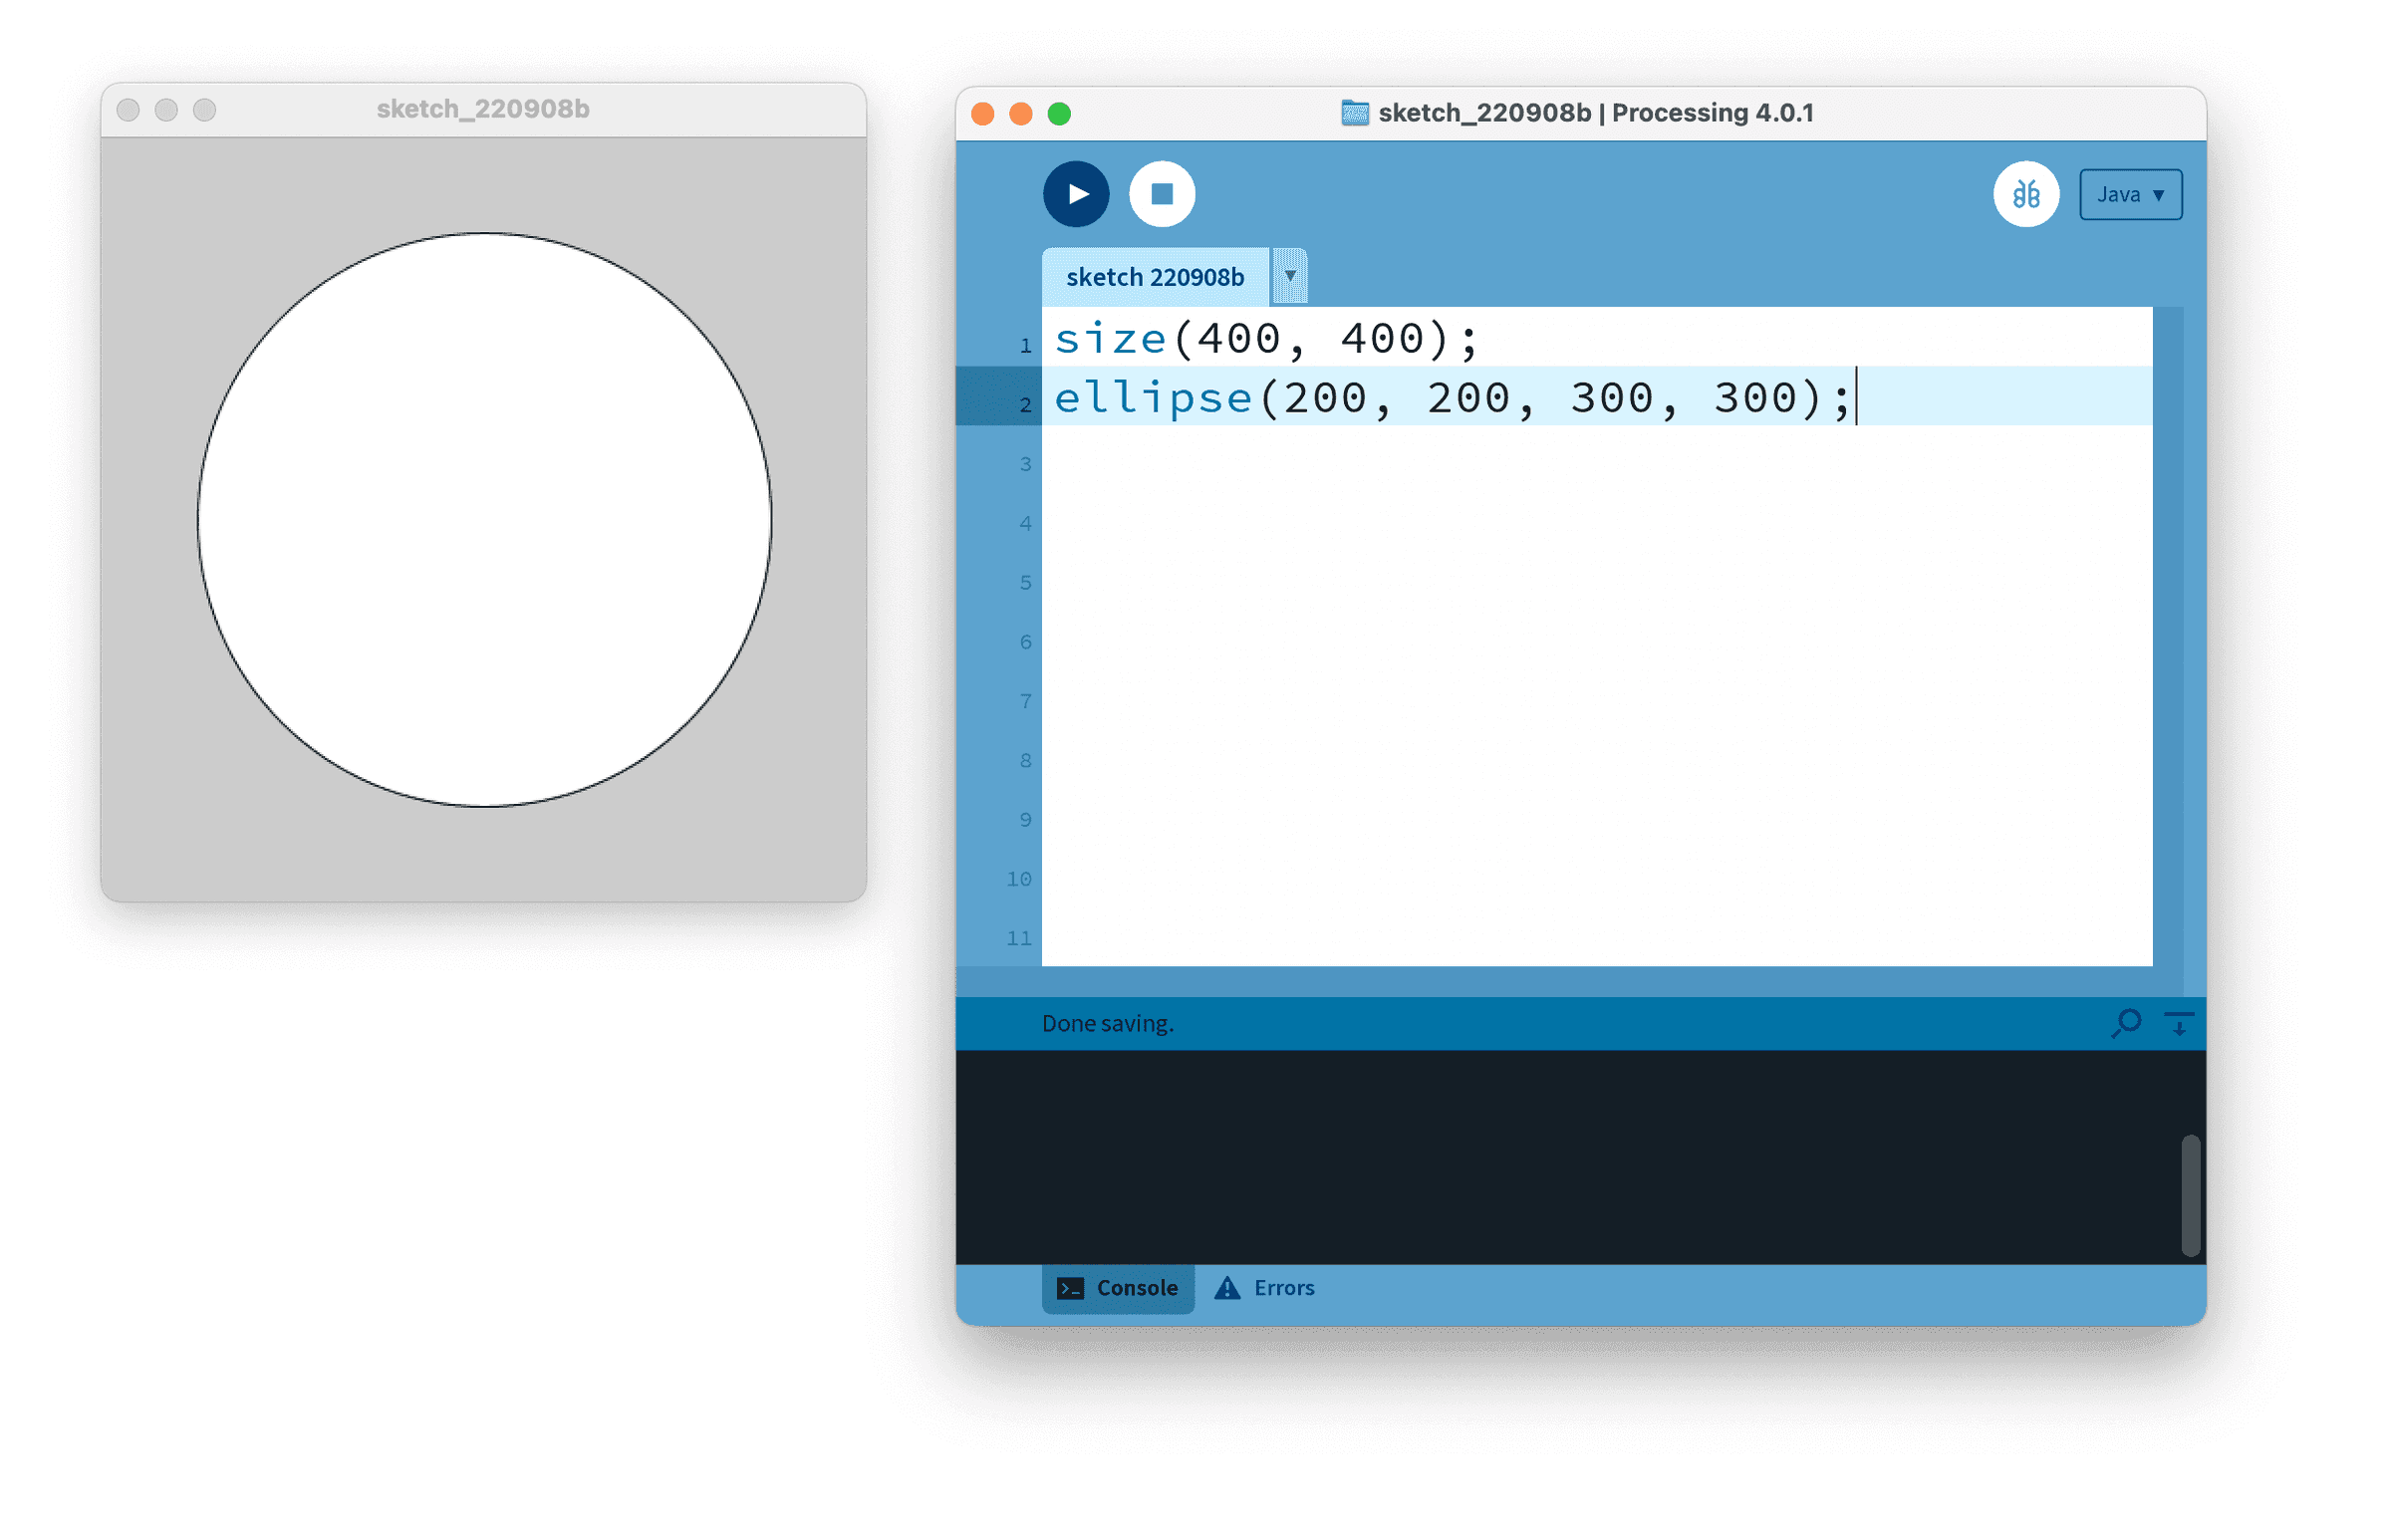
\includegraphics[width=1\textwidth]{images/processing_ide.png} 
%     \caption{Processing IDE \parencite{reasProcessingIDE2015}}
%     \label{fig:processing_ide_screenshot}
%   \end{figure}
  
\subsection{A culture of workshops}

\begin{figure}[h] 
    \centering 
    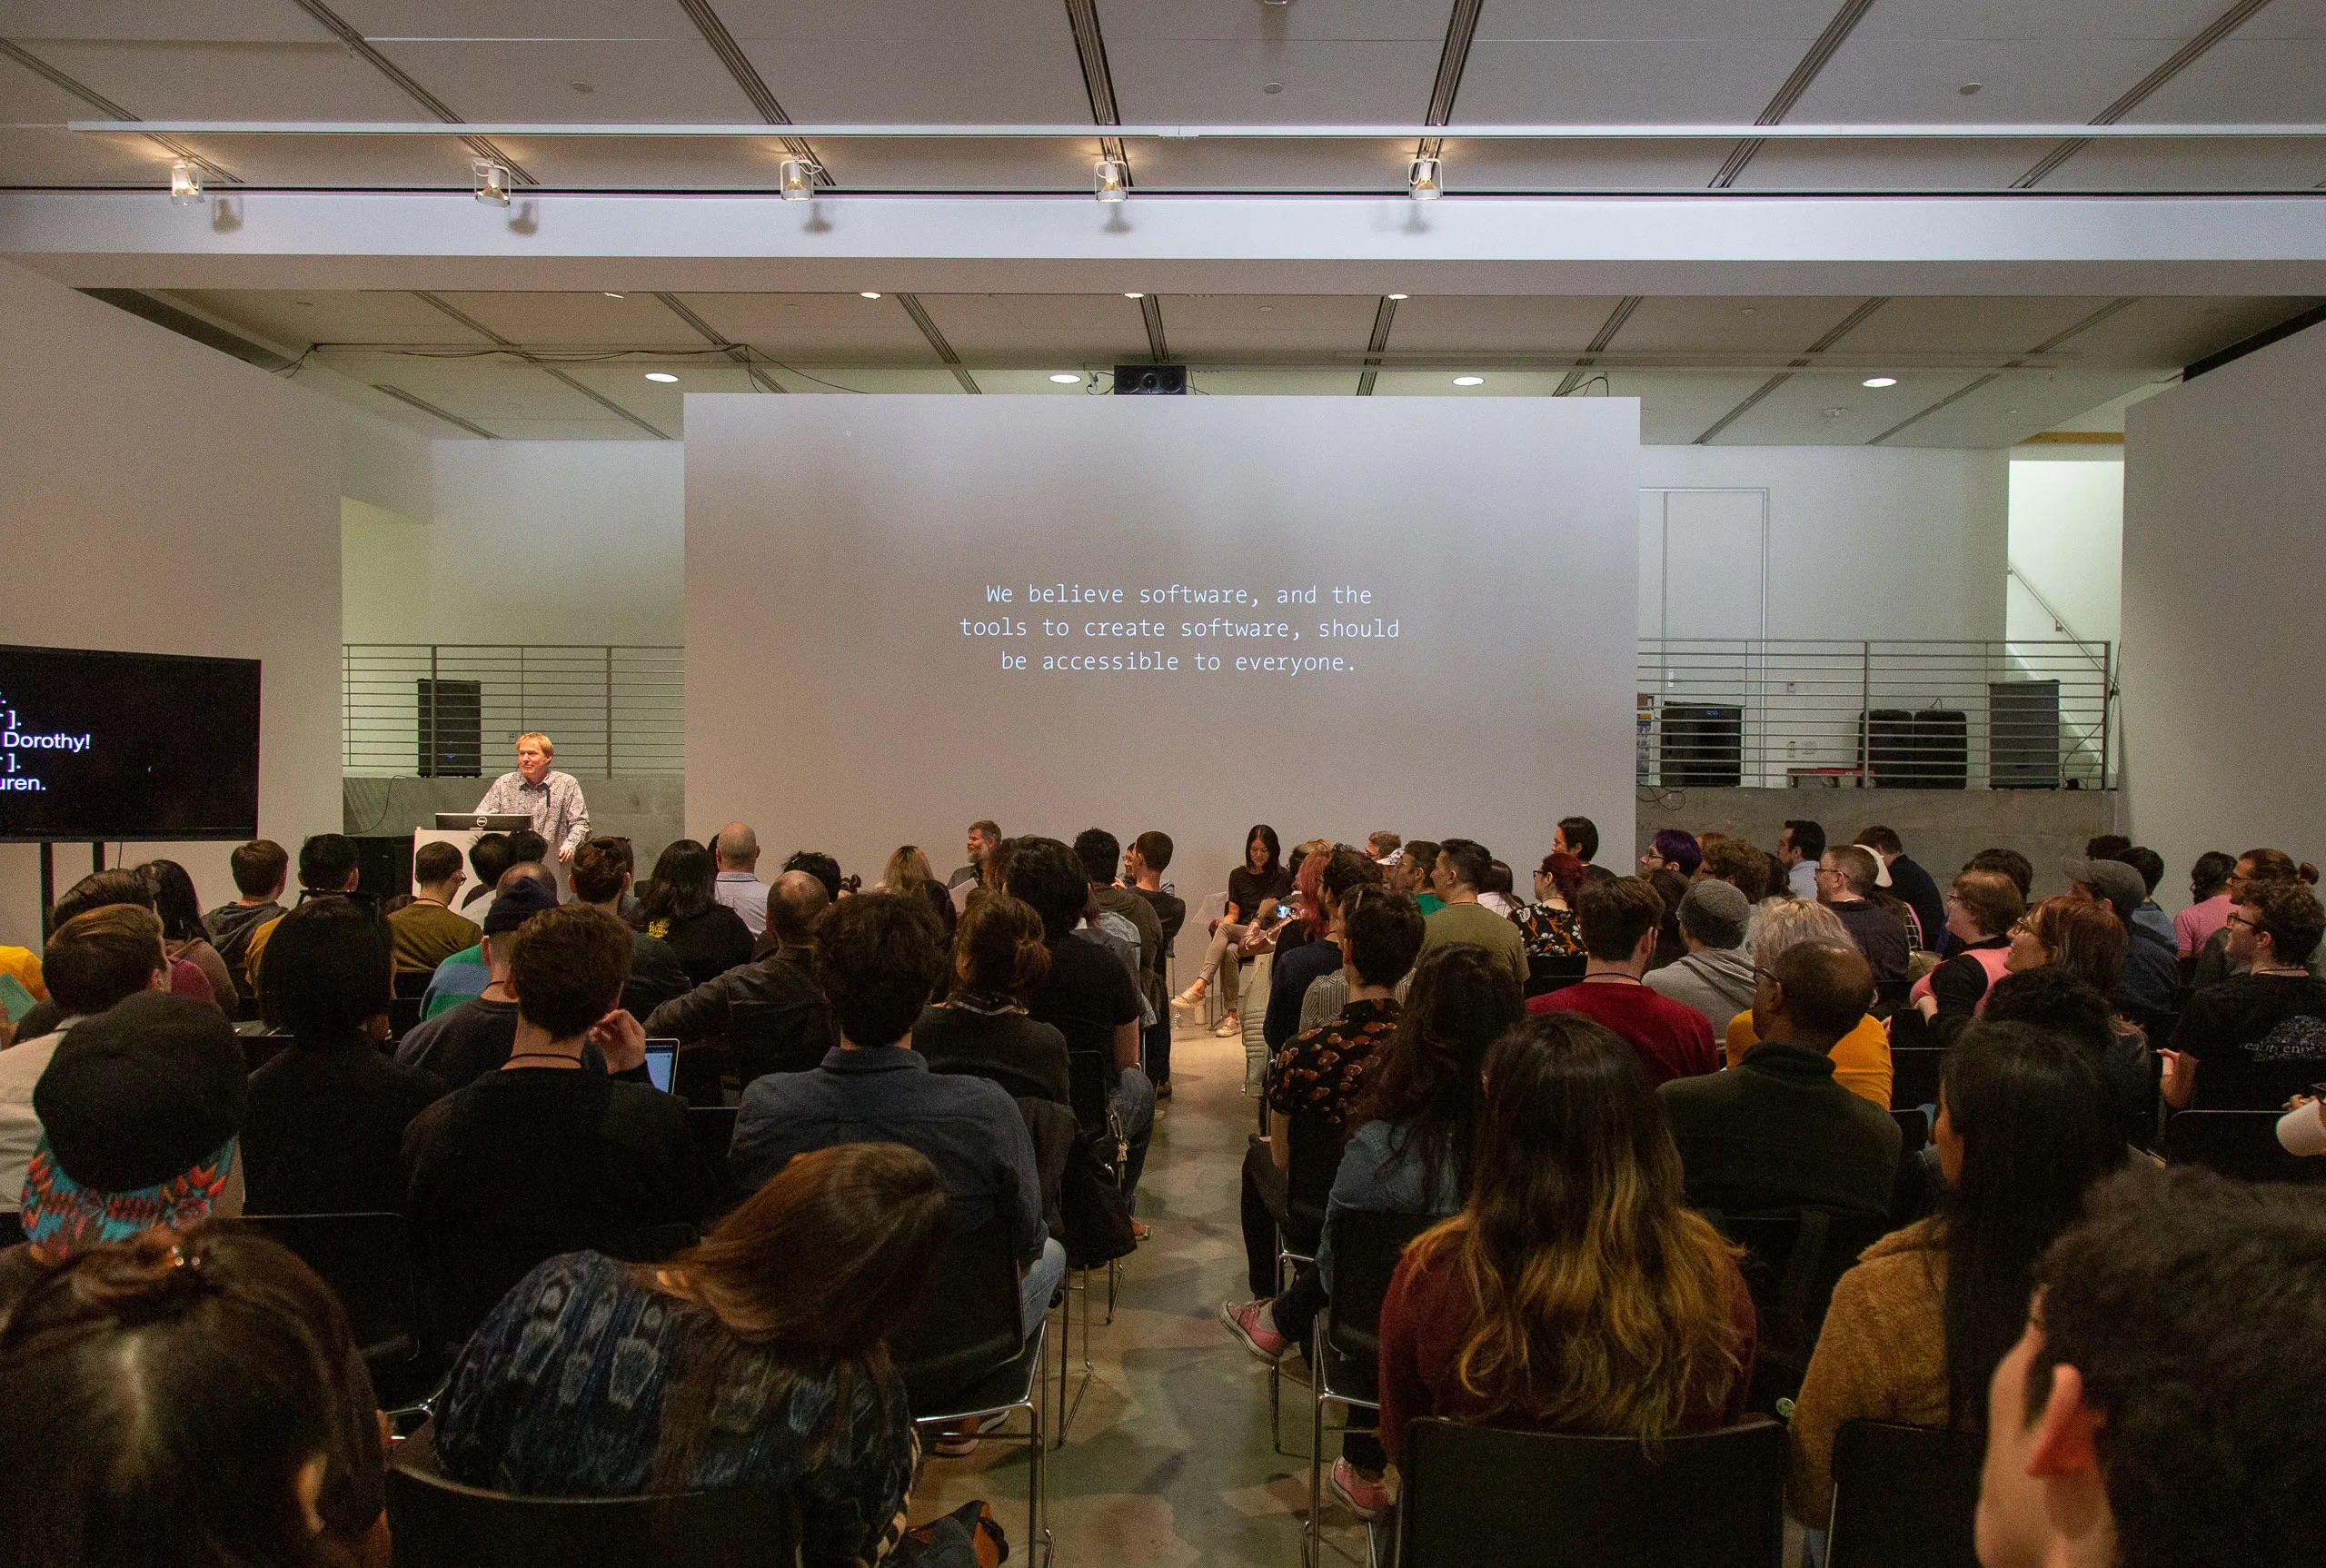
\includegraphics[width=1\textwidth]{images/pcd_la_2019.jpeg} 
    \caption[Ben Fry at PCD 2018]{Ben Fry with conference attendees. Source: \citefield{guptaBenFryConference2018}{author}, Medium, \citeyear{guptaBenFryConference2018}.}
\end{figure}

\subsection{An ecosytem of libraries}
An important milestone in the Processing ecosystem was the introduction of libraries. These libraries extended the functionalities of the base platform, thereby attracting a broader range of users and contributors. Such an analysis not only sheds light on the diversification of the project but also identifies key contributors and library authors who could potentially be sought out for qualitative interviews. The identification of these contributors adds another layer to our understanding of community participation.

\changepapersize{305.3mm:210mm}
\customtag{largepage}

\begin{figure}
    \includesvg[pretex=\sffamily\fontsize{5.58pt}{8pt}\selectfont, width=1\textwidth, keepaspectratio]{images/figure-libraries.svg}
    \caption{Distribution of Libraries in the Processing Project}
    \label{figure:libraries}  
\end{figure}

\defaultareasettings

\subsection{Processing Foundation}

The Processing Foundation was established in 2012 by Casey Reas, Ben Fry, and Daniel Shiffman with the primary objective of sustaining the software's development and broadening its reach. According to Fry and Reas, ``The vast majority of the code is written by the same small number of people volunteering their time — there are no paid full-time developers'' \parencite[p.~13]{fryModernPrometheusHistory2018}.

\begin{figure}[h]
    \centering
    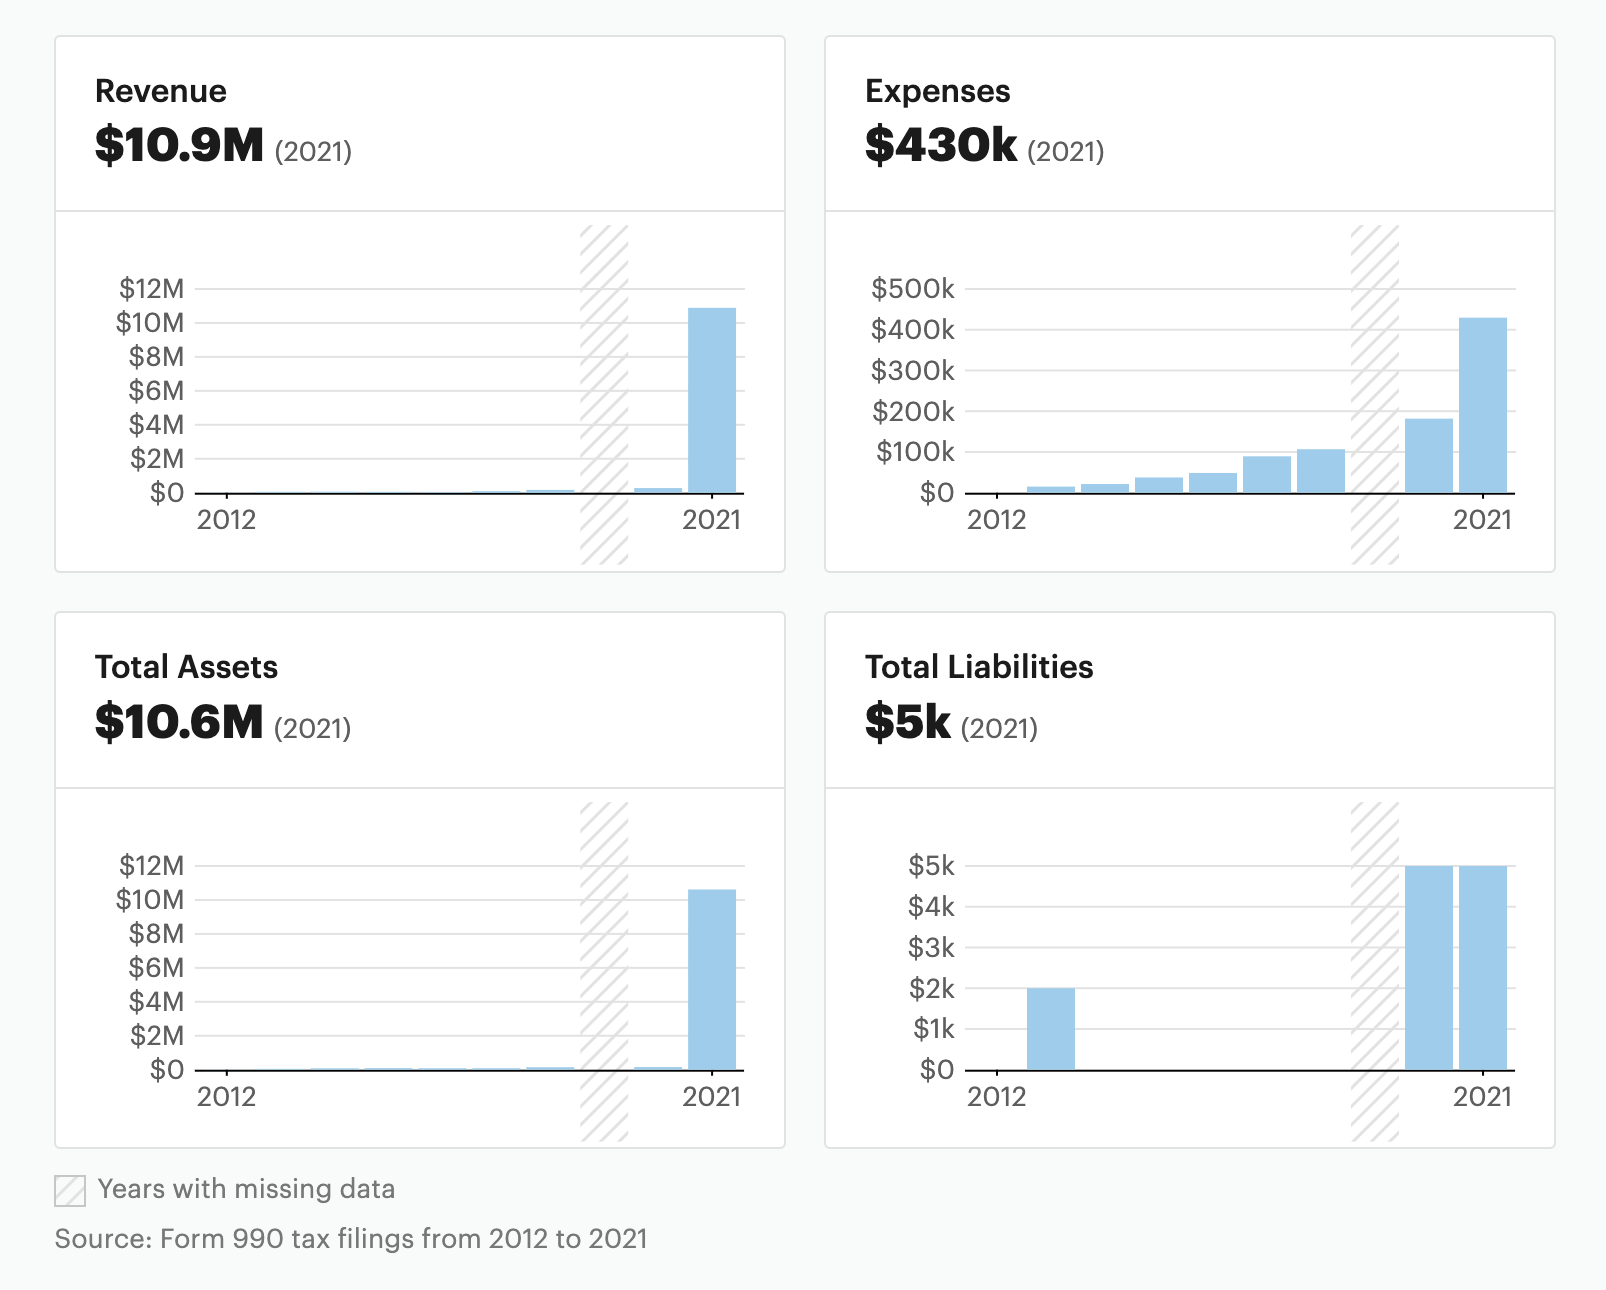
\includegraphics[width=0.9\textwidth]{images/foundation-finances.png} 
    \caption{Financial growth of the Processing Foundation over the years Source: \parencite{ProcessingFoundationNonprofit2013}}
    \label{fig:foundation-finances}
\end{figure}

As shown in Figure~\ref{fig:foundation-finances}, the foundation's revenue has experienced modest growth, increasing from \$11,235 to \$273,520. Remarkably, it reached a peak revenue of \$10,889,998 in the fiscal year 2021. Throughout its history, the principal source of funding for the foundation has predominantly come from contributions. 

However, the allocation of these funds has been a point of contention within the organization. Most notably, a public disagreement in 2023 led to the resignation of Ben Fry, a long-standing board member and contributor. It should be noted that Fry's perspective on the matter was not universally accepted among the foundation's other founding members. \parencite{benfry[@ben_fry]HaveMadeExtremely2023} \parencite{caseyreas[@reas]EarlierThisWeek2023} \parencite{danielshiffman[@shiffman]WouldPostNote2023}

